\documentclass[12pt]{article}

\usepackage{answers}
\usepackage{setspace}
\usepackage{graphicx}
\usepackage{enumitem}
\usepackage{multicol}
\usepackage{mathrsfs}
\usepackage[margin=1in]{geometry} 
\usepackage{amsmath,amsthm,amssymb}
\usepackage{pgfplots}
\pgfplotsset{compat=1.15}
 
\newcommand{\N}{\mathbb{N}}
\newcommand{\Z}{\mathbb{Z}}
\newcommand{\C}{\mathbb{C}}
\newcommand{\R}{\mathbb{R}}

\DeclareMathOperator{\sech}{sech}
\DeclareMathOperator{\csch}{csch}
 
\newenvironment{theorem}[2][Theorem]{\begin{trivlist}
\item[\hskip \labelsep {\bfseries #1}\hskip \labelsep {\bfseries #2.}]}{\end{trivlist}}
\newenvironment{definition}[2][Definition]{\begin{trivlist}
\item[\hskip \labelsep {\bfseries #1}\hskip \labelsep {\bfseries #2.}]}{\end{trivlist}}
\newenvironment{proposition}[2][Proposition]{\begin{trivlist}
\item[\hskip \labelsep {\bfseries #1}\hskip \labelsep {\bfseries #2.}]}{\end{trivlist}}
\newenvironment{lemma}[2][Lemma]{\begin{trivlist}
\item[\hskip \labelsep {\bfseries #1}\hskip \labelsep {\bfseries #2.}]}{\end{trivlist}}
\newenvironment{exercise}[2][Exercise]{\begin{trivlist}
\item[\hskip \labelsep {\bfseries #1}\hskip \labelsep {\bfseries #2.}]}{\end{trivlist}}
\newenvironment{solution}[2][Solution]{\begin{trivlist}
\item[\hskip \labelsep {\bfseries #1}]}{\end{trivlist}}
\newenvironment{problem}[2][Problem]{\begin{trivlist}
\item[\hskip \labelsep {\bfseries #1}\hskip \labelsep {\bfseries #2.}]}{\end{trivlist}}
\newenvironment{question}[2][Question]{\begin{trivlist}
\item[\hskip \labelsep {\bfseries #1}\hskip \labelsep {\bfseries #2.}]}{\end{trivlist}}
\newenvironment{corollary}[2][Corollary]{\begin{trivlist}
\item[\hskip \labelsep {\bfseries #1}\hskip \labelsep {\bfseries #2.}]}{\end{trivlist}}
 
\begin{document}
 
% --------------------------------------------------------------
%                         Start here
% --------------------------------------------------------------
 
\title{Problem Set 1}%replace with the appropriate homework number
\author{Basil R. Yap\\ %replace with your name
40.316 Game Theory - Term 8} %if necessary, replace with your course title
 
\maketitle
%Below is an example of the problem environment

% Question 1
\begin{figure}[h!]
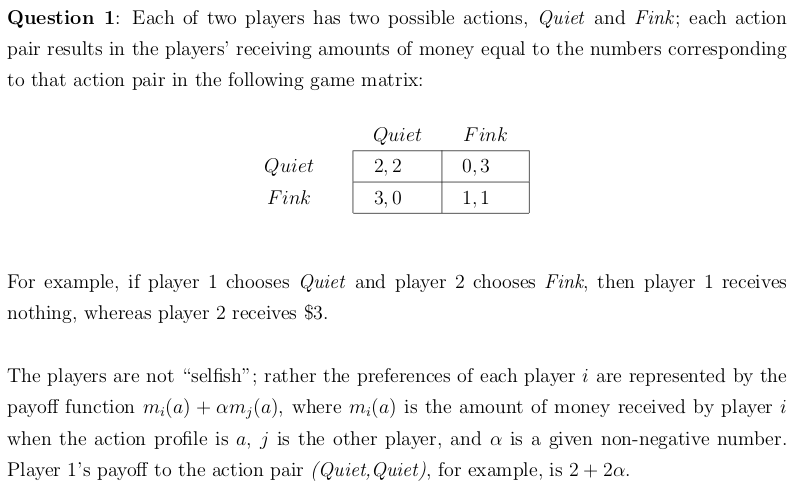
\includegraphics[width=\linewidth]{./assets/201805201632.png}
\end{figure}

\begin{enumerate}[label=\alph*)]
\item Formulate a strategic game that models this situation in the case $\alpha = 1$. Is this game the \textit{Prisoner’s Dilemma}?
\item Find the range of values of $\alpha$ for which the resulting game is the \textit{Prisoner’s Dilemma}.
\end{enumerate}

\begin{solution}{}~
\begin{enumerate}[label=\alph*)]
\item \begin{itemize}
\item Players: Row Player and Column Player
\item Actions: Quiet or Fink
\item Pay-off matrix:\\
\begin{tabular}{| c || c | c |}\hline
 & \textit{Quiet} & \textit{Fink} \\
 \hline\hline
 \textit{Quiet} & $(2+2\alpha,2+2\alpha)$ & $(3\alpha,3)$\\
 \textit{Fink} & $(3,3\alpha)$ & $(1+\alpha,1+\alpha)$\\
 \hline
\end{tabular}
\end{itemize}

When $\alpha=1$, the game is not a \textit{Prisoner's Dilemma}.\\
$u(\textit{Quiet},\{\textit{Quiet},\textit{Fink}\})$ is the dominant strategy for both players, regardless of the other player's decision.
\item For the game to be a \textit{Prisoner's Dilemma},\\
$u(\textit{Quiet},\textit{Quiet})>u(\textit{Fink},\textit{Fink})>u(\textit{Quiet},\textit{Fink})$ for both players.
\begin{gather*}
2+2\alpha>1+\alpha>3\alpha\\
2+\alpha>1>2\alpha\\
2+\alpha>1\text{ is trivial, because }\alpha\geq0\\
1>2\alpha\\
\alpha<\frac{1}{2}
\end{gather*}
The game is a \textit{Prisoner's Dilemma}, when $0\leq\alpha<\frac{1}{2}$
\end{enumerate}
\end{solution}

% Question 2
\begin{figure}[h!]
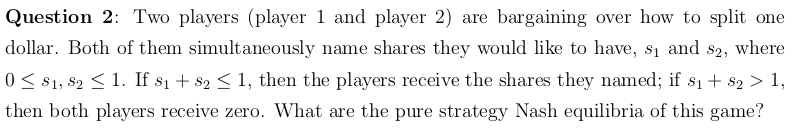
\includegraphics[width=\linewidth]{./assets/201805201646.png}
\end{figure}

\begin{solution}{}~\\

Pay-off Function:\\

$
u_i(s_i)=\left\{\begin{array}{ll}
s_i & \text{If }s_1+s_2\leq1\\
0 & \text{Otherwise}
\end{array}\right.\ \ \ \ \forall i\in\{1,2\}$\\

From the pay-off function, we can get the best response function:\\

$BR_i(s_j)=1-s_j\ \ \ \ \forall i,j\in\{1,2\}$\\

Best Response Graph:\\

\begin{tikzpicture}
\begin{axis}[
    axis lines = left,
    xlabel = {$s_2$},
    ylabel = {$s_1$},
    xmax = 1.2,
    ymax = 1.2
]
%Below the red parabola is defined
\addplot [
    domain=0:1, 
    samples=100,
    color=blue
]
{1-x};
\end{axis}
\end{tikzpicture}

Therefore, the Nash equilibria can be found at:\\

$(s_1,s_2)\ \ \forall s_1,s_2\text{ where }s_1+s_2=1$
\end{solution}

% Question 3
\begin{figure}[h!]
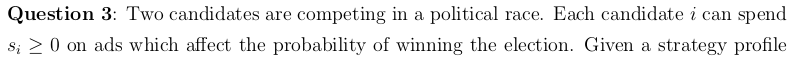
\includegraphics[width=\linewidth]{./assets/201805201648.png}
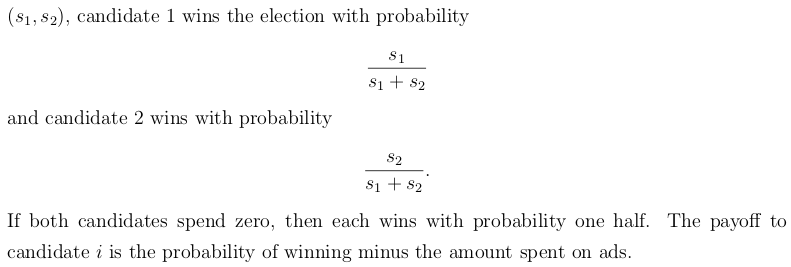
\includegraphics[width=\linewidth]{./assets/201805201649.png}
\end{figure}

\begin{enumerate}[label=\alph*)]
\item Write an expression for the payoff function of candidate 1.
\item Solve for the best response function of each candidate.
\item Find the pure strategy Nash equilibrium.
\end{enumerate}

\begin{solution}{}~\\
\begin{enumerate}[label=\alph*)]
\item Pay-off function for Candidate 1:\\

$$u_1(s_1)=\frac{s_1}{s_1+s_2}-s_1$$
\item Pay-off function for both Candidates:\\
\begin{align*}
u_i(s_i)&=\frac{s_i}{s_1+s_2}-s_i\\
&=\frac{s_i-s_i(s_1+s_2)}{s_1+s_2}\ \ \ \ \forall i \in\{1,2\}
\end{align*}
Best Response for both Candidates:\\
\begin{align*}
\nabla u_i(s_i)&=\frac{d}{ds_i}\left(\frac{s_i-s_i^2-s_is_j}{s_i+s_j}\right)\\
&=\frac{(s_i+s_j)(1-2s_i-s_j)-(s_i-s_i^2-s_is_j)}{(s_i+s_j)^2}\\
&=\frac{s_i-2s_i^2-s_is_j+s_j-2s_is_j-s_j^2-s_i+s_i^2+s_is_j}{s_i^2+2s_is_j+s_j^2}\\
&=\frac{-s_i^2+s_j-2s_is_j-s_j^2}{s_i^2+2s_is_j+s_j^2}\\
&=\frac{s_j}{(s_i+s_j)^2}-1\ \ \ \ \forall i,j \in\{1,2\}
\end{align*}
\begin{align*}
\frac{s_j}{(s_i+s_j)^2}-1&=0\\
s_j&=(s_i+s_j)^2\\
\pm\sqrt{s_j}&=s_i+s_j\\
s_i&=-s_j\pm\sqrt{s_j}\\
BR_i(s_j)&=-s_j\pm\sqrt{s_j}\\
&=\sqrt{s_j}-s_j\ \ \ \ \because s_i\geq0
\end{align*}
\pagebreak
\item Best Response Graph:\\

\begin{tikzpicture}
\begin{axis}[
    axis lines = left,
    xlabel = {$s_1$},
    ylabel = {$s_2$},
    ymax = 1
]
\addplot [
    domain=0:1, 
    samples=100,
    color=blue
]
{-x+(x^0.5)};
\addplot[color=red]
 table[
	x=x,
	y=y,
	col sep=comma
] {pset1.csv};
\legend{$BR_1(s_2)$,$BR_2(s_1)$}
\node[label={45:{(0.25,0.25)}},circle,fill,inner sep=2pt] at (axis cs:0.25, 0.25){};
\node[label={45:{(0,0)}},circle,fill,inner sep=2pt] at (axis cs:0, 0){};
\end{axis}
\end{tikzpicture}

Therefore, the Nash equilibria can be found at:\\

(0, 0) and (0.25, 0.25)

\end{enumerate}
\end{solution}

% Question 4
\begin{figure}[h!]
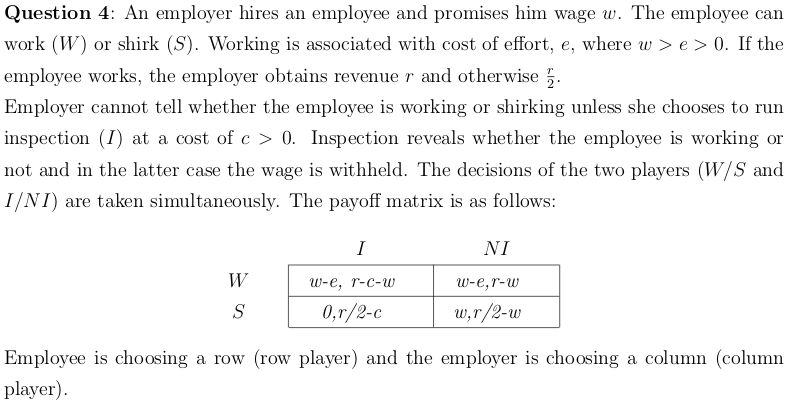
\includegraphics[width=\linewidth]{./assets/201805201650.png}
\end{figure}

\begin{enumerate}[label=\alph*)]
\item Under what condition(s) will this game have a pure strategy Nash equilibrium?
\item Assume the aforementioned condition(s) is (are) not satisfied.  Derive the formulas for
probability of working, $p$ and probability of inspection, $q$ in the mixed strategy Nash equilibrium.
\end{enumerate}

\begin{solution}{}~\\
\begin{enumerate}[label=\alph*)]
\item The game will have a pure strategy Nash Equilibrium when one or more of the following conditions are met:\\

\begin{enumerate}[label=(\roman*)]
\item (W,I)\\
\begin{align*}
w-e&\geq0\text{    // True}\\
r-c-w&\geq r-w\text{    // Not Possible}\\
\end{align*}
\item (W,NI)\\
\begin{align*}
w-e&\geq w\text{    // Not Possible}\\
r-w&\geq r-c-w\text{    // True}
\end{align*}
\item (S,I)\\
\begin{align*}
0&\geq w-e\text{    // Not Possible}\\
\frac{r}{2-c}&\geq\frac{r}{2-w}\text{    // Possible}
\end{align*}
\item (S,NI)\\
\begin{align*}
w&\geq w-e\text{    // True}\\
\frac{r}{2-w}&\geq\frac{r}{2-c}\text{    // Possible}
\end{align*}
\end{enumerate}
(S,NI) is the only pure strategy that can be at Nash Equilibrium.\\
It can only be a Nash Equilibrium when:\\

\begin{tikzpicture}
\begin{axis}[
    axis lines = left,
    axis lines = middle,
    xlabel = {$x$},
    ylabel = {$\frac{1}{2-x}$},
]
\addplot [
    domain=0:1.99, 
    samples=100,
    color=blue
]
{1/(2-x))};
\addplot [
    domain=2.01:4, 
    samples=100,
    color=blue
]
{1/(2-x))};
\end{axis}
\end{tikzpicture}
\begin{align*}
\frac{r}{2-w}&\geq\frac{r}{2-c}\\
2-w&\leq2-c\\
w&\geq c
\end{align*}
$$\text{Where }w,c\neq2\text{ and both }w,c<2\text{ or }w,c>2$$
$$\textbf{OR }w\in[0,2)\text{ and }c\in(2,\infty)$$
\item Expected pay-off for row player given row player's action:\\

\begin{align*}
u_1(W,[q,1-q])&=q(w-e)+(1-q)(w-e)\\
u_1(S,[q,1-q])&=(1-q)w\\
\text{Solve }u_1(W,[q^*,1-q^*])&=u_1(S,[q^*,1-q^*])\\
q^*(w-e)+(1-q^*)(w-e)&=(1-q^*)w\\
q^*w-q^*e+q^*e-e&=0\\
q^*w&=e\\
q^*&=\frac{e}{w}
\end{align*}
Expected pay-off for column player given column player's action:

\begin{align*}
u_2(I,[p,1-p])&=p(r-c-w)+(1-p)(\frac{r}{2-c})\\
u_2(NI,[p,1-p])&=p(r-w)+(1-p)(\frac{r}{2-w})\\
\text{Solve }u_2(I,[p^*,1-p^*])&=u_2(NI,[p^*,1-p^*])\\
p^*(r-c-w)+(1-p^*)(\frac{r}{2-c})&=p^*(r-w)+(1-p^*)(\frac{r}{2-w})\\
-p^*c&=(1-p^*)\left(\frac{r}{2-w}-\frac{r}{2-c}\right)\\
\frac{p^*}{p^*-1}&=\frac{r}{2c-cw}-\frac{r}{2c-c^2}\\
&=\frac{2rc-rc^2-2rc+rcw}{4c^2-2c^3-2c^2w+c^3w}\\
&=\frac{rw-rc}{4c-2c^2-2cw+c^2w}\\
1-p^*&=\frac{4c-2c^2-2cw+c^2w}{rw-rc}\\
p^*&=1-\frac{c}{r}\frac{4-2c-2w+cw}{w-c}\\
&=1-\frac{c}{r}\frac{(2-c)(2-w)}{w-c}
\end{align*}
\end{enumerate}
\end{solution}

% Question 5
\begin{figure}[h!]
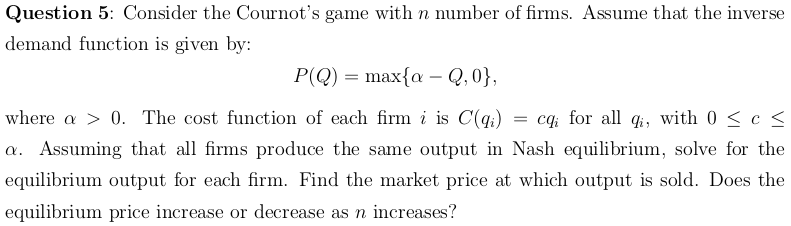
\includegraphics[width=\linewidth]{./assets/201805201651.png}
\end{figure}

\begin{solution}{}~\\
Assuming that all firms produce the same output in Nash Equilibrium.\\
In Nash Equilibrium,\\
\begin{align*}
Q&=nq\text{ where }q=q_i\ \ \ \ \forall i\in[1,n]\\
u_i&=q\times\max\{\alpha-nq,0\}-cq
\end{align*}
$$u_i=\left\{\begin{array}{ll}
q(\alpha-nq)-cq & \text{If }\alpha-nq>0\\
-cq & \text{Otherwise}
\end{array}\right.$$
Equilibrium output for all firms:\\

\begin{align*}
\frac{du_i}{dq}&=\frac{d}{dq}(q(\alpha-nq)-cq)\\
&=\alpha-2nq-c\\
\text{Solve for }q^*&\text{ when }\frac{du_i}{dq}=0\\
0&=\alpha-2nq^*-c\\
2nq^*&=\alpha-c\\
q^*&=\frac{\alpha-c}{2n}
\end{align*}
Market price at Nash Equilibrium:\\

\begin{align*}
P&=\max\{\alpha-nq^*,0\}\\
&=\max\{\alpha-n(\frac{\alpha-c}{2n}),0\}\\
&=\max\{\alpha-\frac{\alpha-c}{2},0\}
\end{align*}
As $n$ increases, there is no change to the equilibrium price.\\
But the optimal production quantity $q^*$ decreases as $n$ increases.
\end{solution}

\pagebreak

% Question 6
\begin{figure}[h!]
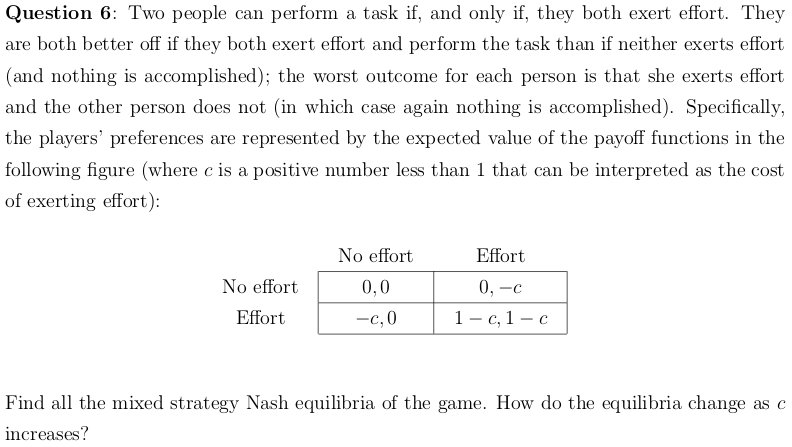
\includegraphics[width=\linewidth]{./assets/201805201652.png}
\end{figure}

\begin{solution}{}~\\
Expected pay-off for row player given row player's action:\\
Let $q$ be the probability of column player picking \textit{No Effort}.

\begin{align*}
u_1(\textit{No Effort}, [q,1-q])&=0\\
u_1(\textit{Effort}, [q,1-q])&=-cq+(1-c)(1-q)\\
\text{Solve }u_1(\textit{No Effort}, [q^*,1-q^*])&=u_1(\textit{Effort}, [q^*,1-q^*])\\
0&=-cq^*+(1-c)(1-q^*)\\
cq^*&=1-q^*-c+cq^*\\
q^*&=1-c
\end{align*}
Expected pay-off for column player given column player's action:\\
Let $p$ be the probability of the row player picking \textit{No Effort}.
$$p^*=1-c$$
$$\because \text{ pay-off matrix is symmetric.}$$

Nash Equilibrium for the game: [($1-c$,$c$),($1-c$,$c$)] for $c\in(0,1)$\\

When $c\in\{0,1\}$, there are two pure strategy Nash Equilibrium,\\
(\textit{No Effort},\textit{No Effort}) and (\textit{Effort},\textit{Effort}).\\

When $c\in(0,1)$, the mix strategy Nash Equilibria exists and \\
tends towards (\textit{Effort},\textit{Effort}) as $c$ increases.
\end{solution}

\end{document}
